\documentclass[border=4pt]{standalone}
\usepackage{fontspec}
\usepackage{amsmath}
\usepackage{unicode-math}
\setmainfont{Latin Modern Roman}
\setmathfont{Latin Modern Math}
\usepackage{pgfplots}
\usepackage{pgfplotstable}
\pgfplotsset{compat=1.18}
\usepackage{tkz-euclide}
\usetikzlibrary{arrows.meta,calc,angles,quotes,patterns,3d,backgrounds}
\definecolor{ink}{HTML}{123428}
\definecolor{asy}{HTML}{475569}
\definecolor{mint}{HTML}{86e0bd}
\tikzset{asym/.style={asy, line width=0.9pt, dash pattern=on 5pt off 3.5pt},
         guide/.style={gray!70, line width=0.6pt, densely dotted},
         dot/.style={circle, inner sep=0pt, minimum size=5pt, draw=white, line width=0.5pt},
         odot/.style={circle, inner sep=0pt, minimum size=5.5pt, fill=white, line width=1pt},
         lab/.style={font=\footnotesize, inner sep=1.5pt, text=ink}}
\begin{document}
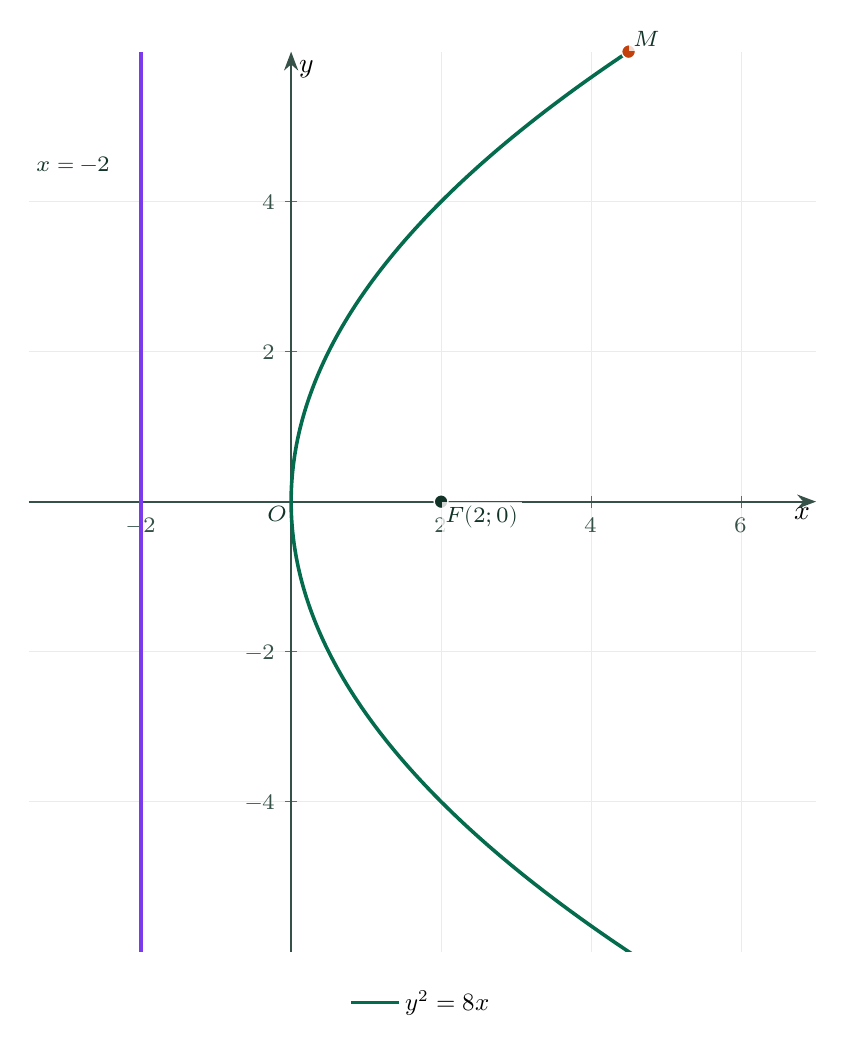
\begin{tikzpicture}
\begin{axis}[
  scale only axis,
  width=10.00cm,
  height=11.43cm,
  axis lines=middle,
  xmin=-3.5, xmax=7, ymin=-6, ymax=6,
  axis line style={draw=ink!85, line width=0.7pt, -{Stealth[length=2.4mm]}},
  xlabel={$x$}, ylabel={$y$},
  xlabel style={at={(ticklabel* cs:1)}, anchor=north east, inner sep=2pt},
  ylabel style={at={(ticklabel* cs:1)}, anchor=north west, inner sep=3pt},
  grid=major, major grid style={draw=gray!16, line width=0.4pt},
  tick style={draw=ink!70},
  ticklabel style={font=\footnotesize, text=ink!85},
  xtick={-2,2,4,6},
  xticklabels={$-2$,$2$,$4$,$6$},
  ytick={-4,-2,2,4},
  yticklabels={$-4$,$-2$,$2$,$4$},
  clip mode=individual,
  every axis plot/.append style={line join=round},
  legend style={at={(0.5,-0.03)}, anchor=north, draw=none, fill=none, font=\small, legend columns=-1, /tikz/every even column/.append style={column sep=10pt}},
  legend cell align=left]
\node[lab, anchor=north east] at (axis cs:0,0) {$O$};
\addplot[color={rgb,255:red,4;green,107;blue,77}, line width=1.3pt, variable=\t, domain=-6.5:6.5, samples=160, smooth] ({\t*\t/8},{\t});
\addlegendentry{$y^{2} = 8x$}
\addplot[color={rgb,255:red,124;green,58;blue,237}, line width=1.3pt, variable=\t, domain=-6:6, samples=2, smooth, forget plot] ({-2+0*\t},{\t});
\node[dot, fill={rgb,255:red,18;green,52;blue,40}] at (axis cs:2,0) {};
\node[lab, anchor=north west, fill=white, fill opacity=0.8, text opacity=1] at (axis cs:2,0) {$F(2; 0)$};
\node[dot, fill={rgb,255:red,194;green,65;blue,12}] at (axis cs:4.5,6) {};
\node[lab, anchor=south west, fill=white, fill opacity=0.8, text opacity=1] at (axis cs:4.5,6) {$M$};
\node[lab] at (axis cs:-2.9,4.5) {$x = -2$};
\end{axis}
\end{tikzpicture}
\end{document}
